\section{Memory management}
\subsection{Manual memory management}
In un linguaggio come il C, il programmatore chiama le funzioni \textbf{malloc} o \textbf{calloc} per scrivere un oggetto sulla memoria. Queste funzioni ritornano un puntatore dell'oggetto che risiede nell'heap. Quando questo oggetto non serve piu il programmatore chiama una \textbf{free} in modo tale da liberare quello spazio della memoria e utilizzarlo per qualcos'altro. \newline Questo tipo di memory management e' chiamato \textbf{explicit deallocation}, il controllo sta tutto nel programmatore, e questo permette di rendere piu facili l'ottimizzazione soprattutto in casi di poca memoria. \newline

\begin{figure}[h!]
  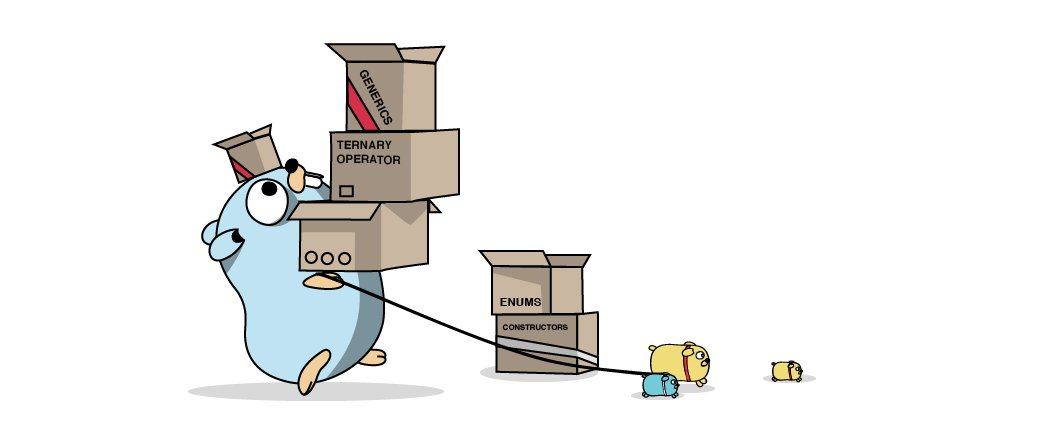
\includegraphics[width=\linewidth]{sections/golang-difficult.jpg}
  \label{fig: go1}
\end{figure}

Questo pero puo creare problemi, per esempio chiamando una \textbf{free} su un oggetto prematuramente, crea un errore di tipo \textbf{dangling pointer}, ovvero puntatori non piu presenti in memoria ma che vengono richiesti lo stesso. \newline
Oppure nel caso il programmatore si dimenticasse di chiamare una \textbf{free} potrebbe incorrere ad un errore di tipo \textbf{memory leak}, ovvero la memoria si riempie fino a non avere piu spazio e quindi crash. \newline

\subsection{Automatic memory management}
Questo viene risolto dai linguaggi come il go che offrono una gestione della memoria automatica, anche chiamata \textbf{garbage collection} che offre diversi vantaggi tra cui: \newline

\begin{itemize}
    \item Aumenta la sicurezza
    \item Portabilita tra i sistemi operativi
    \item Meno codice da scrivere
    \item Codice validato a runtime
\end{itemize}

Ovviamente non e' gratis, il garbage collection costa di piu in termini computazionali, ma permette al programmatore di concentrarsi solamente sulla business logic invece di preoccuparsi a gestire la memoria.
